\documentclass{article}
\usepackage[utf8]{inputenc}
\usepackage{physics}
\usepackage{amsmath}
\usepackage{amssymb}
\usepackage{graphicx}
\usepackage{float}
\usepackage{hyperref}
\hypersetup{
    colorlinks=true,
    linkcolor=blue,
    filecolor=magenta,      
    urlcolor=cyan,
}


\title{Homework 2: Multi-Layer \& Convolutional Neural Networks}
\date{Due October 11, 2019 at 11:59pm}
\author{CS 1470/2470}
\begin{document}

\maketitle

\section{Conceptual Questions}
\begin{enumerate}
\item
Consider the three following 23x23 images of the digit 3. \\

\begin{figure}[H]
    \centering
    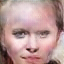
\includegraphics[width=\textwidth]{figs/3.png}
    \label{fig:3}
\end{figure}
Which neural net is better suited for identifying the digit in each image: a convolutional neural net or a feed-forward neural network? Explain your reasoning. (2-3 sentences)

\item
In lecture, you were introduced to the concepts of \emph{translational invariance} and \emph{translational equivariance}.
\begin{enumerate}
    \item What is the difference between these two concepts? \emph{(We expect to see some function notation and text.)}
    \item What part(s) of a convolutional neural network (CNN) with max-pooling, if any, are translationally equivariant, and why? (1-2 sentences)
    \item What part(s) of a CNN with max-pooling, if any, are translationally invariant, and why? (1-2 sentences)
    \item Consider the images of the digit 3 in the previous question. Will a CNN with standard max-pooling (e.g 2x2 pooling) produce the same or different outputs for all of them? Why/why not? How does this relate to translational invariance/equivariance? (hint: remember that the image is 23x23) (2-4 sentences)
\end{enumerate}

\item
Consider the dataset shown in this scatterplot:
\begin{figure}[H]
    \centering
    \includegraphics[width=0.75\textwidth]{figs/hw_image.PNG}
    \label{fig:scatterplot}
\end{figure}
The orange points are labeled with class label 0, and the blue points are labeled with class label 1.
Write out a mathematical expression in terms of the inputs, using linear layers and ReLUs, that will correctly classify all of these points. \emph{(We expect something like $output =....x_1+....x_2$. \\
Hint: Use \url{https://tinyurl.com/y5gayl5b}.)}\\

\item (Optional) Have feedback for this assignment? Found something confusing? We'd love to hear from you!

\end{enumerate}


\section{Ethical Implications}
\begin{enumerate}

\item 
Suppose you want to build an app designed for visually-impaired people to help them gain more information about what’s around them; they can take a picture of something, and your app will tell them what’s “in the picture.” 
\begin{enumerate}
\item
Is there anything different in your design and development process from if you were designing a general-purpose image recognition app? \emph{(Hint: while user testing is an important component, also think about what goes into the algorithm itself…)} (2-3 sentences)

\end{enumerate}

\item
Read about \href{https://www.technologyreview.com/s/602955/neural-network-learns-to-identify-criminals-by-their-faces/}{this algorithm}, which claims to predict “criminality” based on people’s faces, and was created by researchers in China. (If interested, you can click through to the arxiv link where the researchers publish a response to criticism \& media about their original paper).
\begin{enumerate}
    \item 
    What factors do the researchers claim contribute to “criminality?” (1-3 sentences)

    \item 
    What’s one potential confounding variable/feature that their algorithm learned? What’s your evaluation of the “effectiveness” of this algorithm? (2-4 sentences)
    
    \item
    If this algorithm were actually deployed, what are the consequences of this algorithm making a mistake (misclassification)? (1-3 sentences)
\end{enumerate}

\end{enumerate}


\section{CS2470-only Questions}

\begin{enumerate}
\item Prove that convolution is equivariant under translation (it’s fine to do this just for 1D convolution).

\item Suppose you have a CNN that begins by taking an input image of size 28x28x3 and passing through a convolution layer that convolves the image using 3 filters of dimensions 2x2x3 with valid padding.
\begin{enumerate}
    \item How many learnable parameters does this convolution layer have?
    \item Suppose that you instead decided to use a fully connected layer to replicate the behavior of this convolutional layer. How many parameters would that fully connected layer have?
\end{enumerate}


    
\end{enumerate}

\end{document}
